\section{La température qui monte}\label{ex:fusion}

Dans un récipient qui contient de l'eau, on a placé un thermomètre. On a relevé la température de l'eau toutes les 10 min.

\begin{center}
	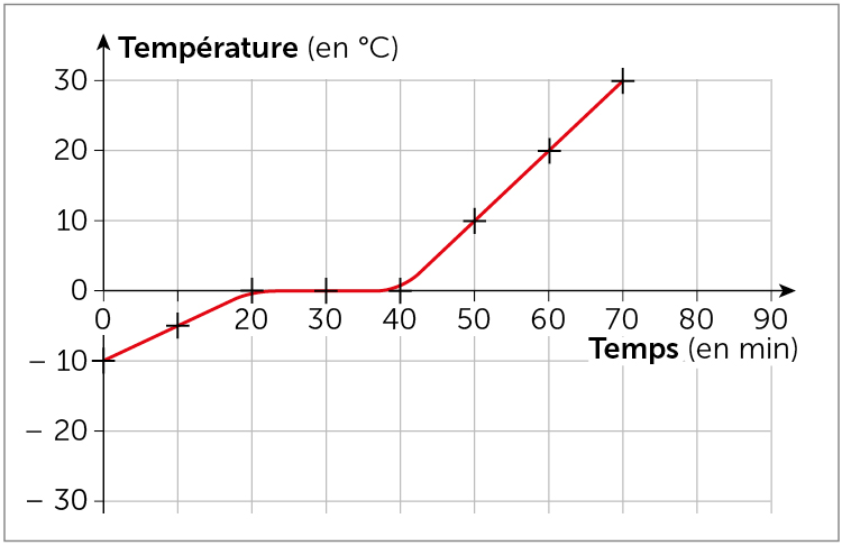
\includegraphics[scale=0.4]{./img/courbe}
\end{center}

\begin{questions}
	\question[2] \'A l'aide de la courbe, indiquer les différents états de l'eau.
	
	\question[1] \`A quel changement d'état cette expérience correspond-elle ? 
\end{questions}